\documentclass{beamer}
\usepackage{amsmath}
\usepackage[utf8]{inputenc}
\usepackage{graphicx}
\usetheme{Warsaw}
\usecolortheme{wolverine}

\title{presentation}
\subtitle{using beamer}
\author{vlnreddy,Aditya Pedavegi }
\date{February 2019}

\begin{document}
\maketitle
\begin{frame}{Question}
Find the product of perpendiculars drawn from the foci of ellipse $(x^2/9) + (y^2/25) = 1$ upon the tangent to it at point $(3/2 ,5\sqrt3/2) $.

 \end{frame}
 
 \begin{frame}{Matrix Interpretation}
 Given equation of ellipse can be written in matrices as
\begin{equation*}
x^T 
\begin{bmatrix}
25 & 0
\\
0 & 9
\end{bmatrix}
x = 225 ....(1)
\end{equation*}
A conic can be expressed in the form of
\begin{equation*}
    x^T V x + 2u^T x + F = 0.....       (2)
\end{equation*}
By comparing (1) and (2), we can say
\begin{equation*}
    V = \begin{bmatrix}
    25 & 0
    \\
    0 & 9
    \end{bmatrix},
    u = 0, F = -225 ....(3)
\end{equation*}
If x is the some vector then
\begin{equation*}
  (p^T V + u^T )x + p^T u + F = 0 ....(4)
\end{equation*}
     is the Tangent vector equation
 \end{frame}
 
 \begin{frame}{Theoritical Computations}
 $$(
\begin{bmatrix}
3/2 & 5\sqrt{3}/2
\end{bmatrix}
\begin{bmatrix}
25 & 0 \\
0 & 9 
\end{bmatrix}
)x + 0 = 225 $$

$$(
\begin{bmatrix}
75/2 & 45\sqrt3/2
\end{bmatrix}
)x = 225 $$
$$\Rightarrow{} T : n^T x = 225$$

$$n = 
\begin{bmatrix}
5/2 \\
3\sqrt3/2
\end{bmatrix}$$

$$e = \sqrt{1-a^2/b^2}$$

$$ e = 4/5 $$
$$ foci = (0,be),(0,-be)$$

$$\Rightarrow{} foci = (0,4),(0,-4)$$
      
\end{frame}

 \begin{frame}{Theoritical Computations}
     Tangent of vector : 
$$\begin{bmatrix}
10 & 6
\end{bmatrix}
\begin{bmatrix}
a \\
b
\end{bmatrix}
 - 225 = 0  $$
 
 let dist1 be the perpendicular distance from s1 \\
 and dist2 be the perpendicular distance from s2 \\
 
 $$A = 
\begin{bmatrix}
 10 & 6\sqrt3
 \end{bmatrix}
\begin{bmatrix}
0\\
4
\end{bmatrix}$$

$$B =
\begin{bmatrix}
10 & 6\sqrt3
\end{bmatrix}
\begin{bmatrix}
0\\
-4
\end{bmatrix}$$
$$C = 
\begin{bmatrix}
10 & 6\sqrt3
\end{bmatrix}
\begin{bmatrix}
3/2 \\
5\sqrt3/2
\end{bmatrix},
D = 
  \sqrt{a^2 + b^2} $$
 \end{frame} 
 
 \begin{frame}{Theoritical Computations}
     dist1 = 
$\frac{||A-C||}{D}\ $\\

dist2 = 
$\frac{||B-C||}{D}\ $
\\
product of distances(D) = dist1 * dist2\\

D = 9
 \end{frame}
 
\begin{frame}{Graphical verification}

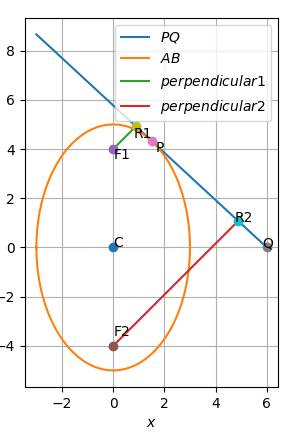
\includegraphics[scale = 0.7]{ellipse_plot.png}
 \end{frame}

\end{document}
